% This is based on "sig-alternate.tex" V1.9 April 2009
% This file should be compiled with V2.4 of "sig-alternate.cls" April 2009
%
% ---------------------------------------------------------------------------------------------------------------
% This .tex source uses a .bib file (from which the .bbl file % is produced).
% REMEMBER HOWEVER: After having produced the .bbl file, and prior to final
% submission, you *NEED* to 'insert' your .bbl file into your source .tex file
% so as to provide ONE 'self-contained' source file.

\documentclass[11pt,twocolumn]{article}
\usepackage[11pt,nocopyright]{sigmin}
\usepackage[square,comma,numbers,sort&compress]{natbib}
\usepackage{times}
\usepackage{microtype}
\usepackage{color}
\usepackage{graphicx}
\usepackage{listings}
\usepackage{multirow}
\usepackage{url}
\lstset{
  numbers=left, frame=lines, tabsize=2, captionpos=b, numberstyle=\tiny,
  columns=fullflexible, showstringspaces=false, basicstyle=\footnotesize\ttfamily,
  extendedchars=true, breaklines=true
}

\setlength{\columnsep}{.25in}

\begin{document}
\title{Challenges and Opportunities in Trusted Computation using Mainstream Computers}
\author{Victor Costan \\ \em MIT CSAIL}
\date{}

\maketitle

\begin{abstract}

We set out to design a system for performing trusted computation on mainstream
desktop and server-class computers. Our system has three mutually distrusting
parties: \textit{a data owner} has some private information, and allows
\textit{a software provider} to perform some computation on the private data,
using hardware resources provided by \textit{an infrastructure owner}. The
computation result is communicated to either the data owner or to the software
provider, in encrypted form.

We aim to build a system that can prevent malicious software from colluding
with either malicious infrastructure, or with another piece of malicious
software running on the same infrastructure, for the purpose of leaking private
data that is not included in the computation result. We rely on a processor's
ability to create a protected execution environment that is isolated from the
system software. Our trusted computing base (TCB) includes the computer's main
processor (CPU), and a \textit{trusted runtime} that verifies and launches the
untrusted software, and mediates its interactions with the software outside the
protected environment. Our TCB does not include the operating system or any
high-level software that runs on the infrastructure.

The main application that we are targeting is enabling heavily regulated
fields, such as the medical and financial industries, to use public clouds and
software as a service (SaaS). While legal consequences make it unlikely that a
public infrastructure or SaaS provider will deliberately act in a malicious
manner, our threat model accounts for skilled attackers who can exploit bugs in
both the infrastructure and the software that performs computation over the
private data.

We have analyzed Intel's most recent proposal for achieving trusted computing,
Software Guard Extensions (SGX), and find that it leaks private data by
exposing the software's memory access patterns to other programs sharing the
infrastructure and to the infrastructure's owners. We aim to find a minimal set
of changes to the SGX proposal that would make it not reveal memory access
patterns, when used in conjunction with our trusted runtime.

\end{abstract}

\section{Motivation}
\label{sec:intro}

In order to achieve certain performance goals, software engineers must often
design systems where the owners of the data being processed are different from
the owners of the computing infrastructure used to process the data, who in
turn might be different from the suppliers of the software that processes the
data. This raises the problem that the data owner must trust both the owner
of the computing infrastructure and the software supplier to handle the data
according to some privacy policy.

The most popular instance of the above problem is cloud computing using public
clouds. For example, CheapoTax, a software provider, might provide tax return
preparation software as a service running on Amazon's public cloud. Users
upload their financial information, encrypted using TLS, to Amazon data
centers, where CheapoTax's computation uses the data to produce tax returns,
which are downloaded by the users in an encrypted form, using TLS. Currently,
the users must trust that neither Amazon nor CheapoTax will record their
private financial information. Users must also hope that neither Amazon's
infrastructure nor CheapoTax's software have bugs that would allow other rogue
actors to obtain the private financial data by running malicious software in
the same public Amazon cloud used by CheapoTax.

Another example of the problem we are aiming to solve is a multiplayer game of
any genre, such as League of Legends \cite{riot2009lol},
World of Warcraft \cite{blizzard2004wow}, StarCraft \cite{blizzard2010sc2}, and
Doom \cite{id2004doom}. The gameplay of many multiplayer games, such as the
ones listed above, rely on the fact that that players can only access a subset
of the game state that is dictated by the units they control. To compensate for
network latencies, many games entrust a player's game client with a superset
of the game state that the user should have access to. For example, in
StarCraft, the game client code running on the players' computers "knows" the
entire state, and is trusted to hide the information that the player should not
have access to \cite{hardy2009cheating}. The other games metioned above also
store information that the player shouldn't access in the game clients, leading
to opportunities for cheating \cite{youtube2013lolcheating}
\cite{youtube2008quake3cheating}.


\subsection{Threat Model}

Our threat model assumes that the infrastructure is shared by multiple ongoing
computations, potentially using software from different mutually distrusting
providers. The operating system and high-level software used to manage the
infrastructure may be malicious, and may cooperate with one or more malicious
pieces of software running on the infrastructure, including the software that
performs computations on the private data that must be protected.

The threat model accurately represents a public cloud. Attackers can rent
resources and run malicious software, as well as run experiments to reveal and
exploit vulnerabilities in the infrastructure software. The programs that run
over the private data can also have vulnerabilities, which can be exploited by
attackers.

In the multiplayer game case, the private data is the full game state, and the
data owner is the same as the software supplier. The infrastructure is the
players' computers. Given that players have an incentive to cheat, it is
reasonable to assume that the infrastructure can behave maliciously. Our system
assumes that the players can exploit any vulnerability available in the game
software. Last, players that desire an unfair advantage can install software
that is specifically designed for cheating, and this software may be running
concurrently with the game software.

Our threat model does not cover attacks that require intimiate knowledge of the
processor's hardware internals. Most importantly, we do not protect against
malicious OS-level software that can abuse a CPU's in-field microcode update
mechanism to create a vulnerability in the processor's security features, or
against attackers that have knowledge of existing vulnerabilities in the CPU.
We also do not protect against attacks that analyze the computer's power
consumption.

Last, the threat model does not include denial of service attacks. Our system
requires the operating system that manages the infrastructure to enable certain
CPU features. We do not trust the operating system, so our system checks for
the features' presence and enablement. If the checks fail, the system refuses
to decrypt private data and to perform any computation. This can lead to a
denial of service attack. At the same time, an attack that compromises the
operating system can cause a denial of service simply by disabling the network
driver, and that cannot be worked around as long as the OS is untrusted.


\section{Background and Related Work}
\label{sec:background}

Arguing about the security of an application running on an mainstream computer
using the x86 platform requires understanding the interactions between
all the parts of an x86 execution environment (protection modes, address
translation hardware, caches). This section provides an overview of these
features from the context of Intel TXT and SGX, touches on existing attacks on
TXT that took advantage of unexpected interactions between the features, and
points out holes in the SGX design that can be used to snoop on a program's
memory access patterns, which can reveal information about the private data
that the program is working on.


\subsection{Software Privilege Levels}
\label{sec:rings}

In an Infrastructure-as-a-Service (IaaS) cloud environment, such as Amazon EC2,
commodity CPUs run software at four different privilege levels: System
Management Mode (SMM), VMX root mode (also described as ring -1), kernel mode
(ring 0) and user mode (ring 3). This section outlines the consequences of a
successfully exploited vulnerability at each privilege level, and sets the
stage for analyzing the SGX protection model.

SMM is intended for use by the motherboard manufacturers to implement features
such as fan control and deep sleep, and/or to emulate missing hardware. SMM
mode is entered by asserting the SMI\# pin on the CPU, which was initially
designed exclusively for hardware use. However, the southbridges on most
motherboards provide a method for the hypervisor and kernel to get the SMI\#
pin asserted\footnote{Most southbridges assert SMI\# when a byte is written to
port 0xb2 via the \textsc{out} opcode}. The SMM code and data are stored in a
memory area called SMRAM, which, in theory, is not readable or writable when
the processor isn't running in SMM, but its protection mechanisms were bypassed
multiple times \cite{duflot2006smm} \cite{rutkowska2008remap}
\cite{wojtczuk2009smm}, and SMM-based rootkits have been demonstrated
\cite{wecherowski2009smm} \cite{wecherowski2009smm}.

IaaS cloud providers allow their customers to run their operating system of
choice in a virtualized environment. Hardware virtualization
\cite{uhlig2005intel}, called Virtual Machine Extensions (VMX) by Intel,
adds support for a \textit{hypervisor} (also called a Virtual Machine Monitor
/ VMM in the Intel documentation) that runs at a higher privilege level
(VMX root mode) than OS kernels, and is responsible for allocating hardware
resources across multiple operating systems that share the same physical
machine. Hypervisor code generally runs at ring 0 in VMX root mode.

The popular Xen hypervisor uses VMX root mode for improved peformance and a
smaller codebase \cite{zhang2008xen}. \cite{mccune2010trustvisor} proposes
using a hypervisor together with Intel TXT's dynamic root of trust for
measurement (DRTM) to implement trusted execution.
\cite{vasudevan2010requirements} argues that a dynamic root of trust mechanism,
like Intel TXT, is necessary to ensure a hypervisor's integrity. Unfortunately,
any SMM attack can be used to compromise Intel TXT \cite{wojtczuk2009txt}, and
the TXT implementation is complex enough that security vulnerabilities have
been found \cite{wojtczuk2009txt2} \cite{wojtczuk2011txt}.

Mainstream operating systems have monolithic kernels that include device
drivers, filesystem code, networking stacks, and video rendering functionality,
and run at ring 0 (kernel mode). Application code, such as a Web server or
a game client, runs at ring 3 (user mode). Software running inside an SGX
enclave (isolated environment) also executes at ring 3. The OS kernel, running
at ring 0, is responsible for scheduling the execution of code inside enclaves
and for allocating hardware resources (such as RAM) to the enclaves. In IaaS
cloud environments, the virtual machine images provided by customers run in VMX
non-root mode, so the kernel runs in VMX non-root ring 0, and the application
code runs in VMX non-root ring 3. SGX is compatible with VMX, and the
hypervisor is responsible for virtualizing a processor's SGX capabilities.

The monolithic kernel design leads to many opportunities for security
vulnerabilities in kernel code. For example the Linux kernel has had a
significant number of vulnerabilities patched every year, for the past 10 years
\cite{cvedetails2014linux} \cite{chen2011linux}. Also, a successful attack on
SMM or the hypervisor trivially translates into a compromised kernel. SGX
accounts for the possibility of a compromised kernel or hypervisor with an
attestation mechanism covering an enclave's contents, and with a hardware
isolation mechanism for the software inside the enclave. In \S \ref{sec:sgx},
we argue that SGX, as it is currently documented in \cite{intel2013sgxmanual},
appears to provide integrity for the software inside the enclave, but
definitely does not provide privacy, as a compromised SMM, hypervisor, or OS
kernel can obtain the enclave's memory access patterns at high granularity.


\subsection{Address Translation}
\label{sec:paging}

Recent commodity CPUs have many address translation modes, in order to run
legacy software dating back to 1990 natively. This section only addresses the
modes used in modern 64-bit operating systems and 64-bit cloud environments.
\cite{jacob1998virtual} describes the generic concepts and applications of
address translation.

64-bit desktop operating systems use the addressing mode called IA-32e in
Intel programming manual \cite{intel2013manual}, which translates 48-bit
\textit{virtual addresses} into \textit{physical addresses} of at most 52
bits\footnote{The size of a physical address is CPU-dependent, and is 40 bits
for recent desktop CPUs and 44 bits for recent high-end server CPUs.}. The
bottom 12 bits of a virtual address are not changed by the translation. The top
36 bits are grouped into four 9-bit indexes used to navigate a data structure
called \textit{the page tables}. Despite its name, the data structure closely
resembles a perfectly balanced 512-ary search tree where the nodes do not store
keys. Each node is an array of 512 8-byte entries that contain the physical
addresses of the next-level children as well as some flags. The address of the
root node is stored in the CR3 register. The arrays in the last-level nodes
contain the physical addresses that are the result of the address translation.

Hardware virtualization (used in cloud computing) allows a hypervisor to run
multiple operating systems concurrently using the same physical memory, by
adding another layer of address translation. When extended page tables (EPT)
are enabled, the process above is used to translate from a virtual address into
a \textit{guest-physical address}. The translation from guest-physical
addresses to actual physical addresses uses the same process as above, except
the physical address of the root node is stored in a virtual machine control
structure.

Each entry in the page tables has some boolean flags, in addition to the
pointer to the next level. The following flags are particularly interesting for
our goals. The \textit{present} (P) flag is set to 0 to indicate pages that
have been evicted from RAM to a cheaper and slower storage medium. When address
translation encounters a page table entry where P is 0, the CPU generates a
page fault (\#PF), and the OS kernel is responsible for loading the page back
into RAM and resuming execution. If an extended page table (EPT) entry has the
P flag set 0, the CPU performs a VM exit, and the hypervisor has an opportunity
to bring the page into RAM. The \textit{accessed} (A) flag is set to 1 by the
CPU whenever the address translation machinery reads a page table entry, and
the \textit{dirty} (D) flag is set to 1 by the CPU when an entry is accessed by
a memory write operation. The A and D flags give the hypervisor and OS kernel
insight into application memory access patterns, providing the input for the
algorithms that select which pages get be evicted from RAM.

Page table entries have flags that provide access control, in addition to the
flags supporting page swapping. The interesting flags are the \textit{writable}
(W) flag, which can be set to 0 to prohibit\footnote{Writes to non-writable
pages result in general protection faults (\#GP).} memory writes to a page, and
the \textit{disable execution} (XD) flag, which can be set to 0 to prevent
instruction fetches from a page.

Address translation applies to the software running in an SGX enclave
(isolated environment). This means that both the OS kernel and the hypervisor
have an impact over the mapping of virtual addresses to physical addresses, and
either of them can take advantage of the features above to obtain the SGX
application's memory access pattern, at page granularity, as detailed in
\S \ref{sec:sgx_leaks}.


\subsection{CPU Caches}
\label{sec:caching}

Desktop-class multi-core commodity CPUs have three levels of cache memory. Each
core has its own L1 and L2, and all cores share an L3 cache. All cache levels
are located on the CPU die so, according to our threat model, they can be
trusted. In particular, we can assume that software memory reads and writes for
locations that are already cached (and therefore do not generate DRAM requests)
cannot be directly observed by an attacker. This requires that the software's
memory is confired to be cacheable with a write-back policy, and our system
accounts for this requirement.

Cache accesses can be indirectly observed by various timing attacks
\cite{banescu2011cache}, by malicious software that time-shares a CPU or a core
with the targeted software and takes advantage of a specific cache's layout
and replacement algorithms. Our system prevents against these attacks, also by
taking advantage of some details of the cache implementation on commodity CPU
processors. This section describes the aspects that we rely on.
\cite{smith1982cache}, \cite{patterson2013architecture} and
\cite{hennessy2012architecture} all provide good backgrounds on low-level cache
implementation concepts.

The \textit{cache line} is the atomic unit of data transfer between the caches
and the main memory. The cache line size is always a power of two. Assuming
$n$-bit memory addresses and a cache line size of $2^{l}$ bytes, the lowest
$l$ bits of a memory address are an offset into a cache line, and the highest
$n - l$ bits determine the cache line that is used to store the data at the
memory location. All recent processors have 64-byte cache lines.

The L1 and L2 caches in recent processors are multi-way set-associative with
direct set indexing. An $w$-way set-associative cache has its memory divided
into \textit{sets}, where each set has $w$ lines. A memory location can be
cached in any of the $w$ lines in a specific set that is determined by the
highest $n - l$ bits of the location's memory address. Direct set indexing
means that the $S$ sets in a cache are indexed from $0$ to $S - 1$, and a
memory location is cached in the set with index
$address_{n - 1 \ldots n - l} \bmod S$. In the common case where the number of
sets in a cache is a power of two, so $S = 2^{s}$, the lowest $l$ bits in an
address make up the cache line offset, the next $s$ bits are the set index.
The highest $n - s - l$ bits in an address are not used when selecting where a
memory location will be cached.

According to the CPUID instruction results and the Intel programming manuals
\cite{intel2013manual}, the L3 cache of recent processors does not use direct
set indexing, and instead uses a "complex" indexing scheme. The manuals do not
describe the scheme, so our system cannot rely on the L3 cache. Due to the lack
of a specification, our system must treat the L3 cache as untrusted memory.
This is rather unfortunate because, although the shared aspect of the L3 cache
would introduce additional complexity in a design, its large size (30MB on
high-end CPUs, compared to 256KB of per-core L2 cache) would make "taming" this
last level of cache memory very attractive.

Address translation (described in \S \ref{sec:caching}) requires 4 memory
accesses for a 64-bit bare-metal kernel, and 8 memory accesses when a
hypervisor is present. To achieve high clock speeds, the CPU caches address
translations in a TLB (translation look-aside buffer). To make L1 caches as
fast as possible, set lookup does not depend on TLB lookup, so the set index in
an L1 cache can only use the address bits that are not impacted by address
translation. Given a page size $P = 2^{p}$ bytes, this means that
$l + s \le p$. In the x86 architecture $p = 12$, and all recent processors have
64-byte cache lines ($l = 6$) and 64 sets ($s = 6$).

The L2 cache in recent Intel processors is known to use physical indexing
\cite{patterson2013architecture}. The indexing method is not documented in
Intel's manuals and is not reported by the CPUID instruction, as it is
considered to be an implementation detail. However, the indexing mehtod
determines the set index for a given memory location, and knowing which memory
addresses are stored in the same set is crucial for mounting and defending
against cache timing attacks.

\section{Design Approach}
\label{sec:design}

Our system aims to offer the same integrity guarantees as SGX, but also provide
full privacy for the code executing inside a protected container, by hiding the
code's memory access patterns against the attacks described in \S
\ref{sec:sgx_leaks}.

We rely on a protected container that is very similar to an SGX enclave. We
pursue two avenues for designing the container. We will explore a minimal set
of SGX modifications that would prevent against memory access patterns leaking
from enclave execution. We will also explore a clean-slate design that
specifies a minimal set of additions to a RISC architecture resulting in a
protected contained that meets our threat model.

In our system, the infrastructure's kernel or hypervisor is responsible for
creating the protected container and loading our trusted runtime into it. The
runtime loads the untrusted software and private data, and verifies that the
protected container was set up correctly, and that the untrusted software
only interacts with the outside world through the runtime. For example, all
the software's memory access instructions must be replaced by calls into our
runtime's memory manager, which that implements an oblivious RAM (ORAM)
protocol \cite{stefanov2013path} that hides the software's memory access
patterns.

SGX has an attestation mechanism that uses a signature of the enclave's initial
contents to set up a secure communication channel between a remote user and
the software running inside the enclave. In our system, the signature only
covers our trusted runtime, reflecting the fact that the software computing on
the private data is not in the TCB.


\subsection{The Memory Manager}

The memory manager sets up the L2 cache as a trusted scratchpad. We target the
L2 cache because we trust all the components on the CPU die, and the L2 cache
is the largest on-die cache where we understand the set indexing method
(\S \ref{sec:caching}).

The memory manager partitions the sets of the L2 cache into scratchpad sets and
real memory sets. The untrusted software's code and data must only occupy
addresses that map to the real memory sets. The protected environment must also
have a memory area that maps to the scratchpad sets.

\begin{figure}[hbtp]
  \center{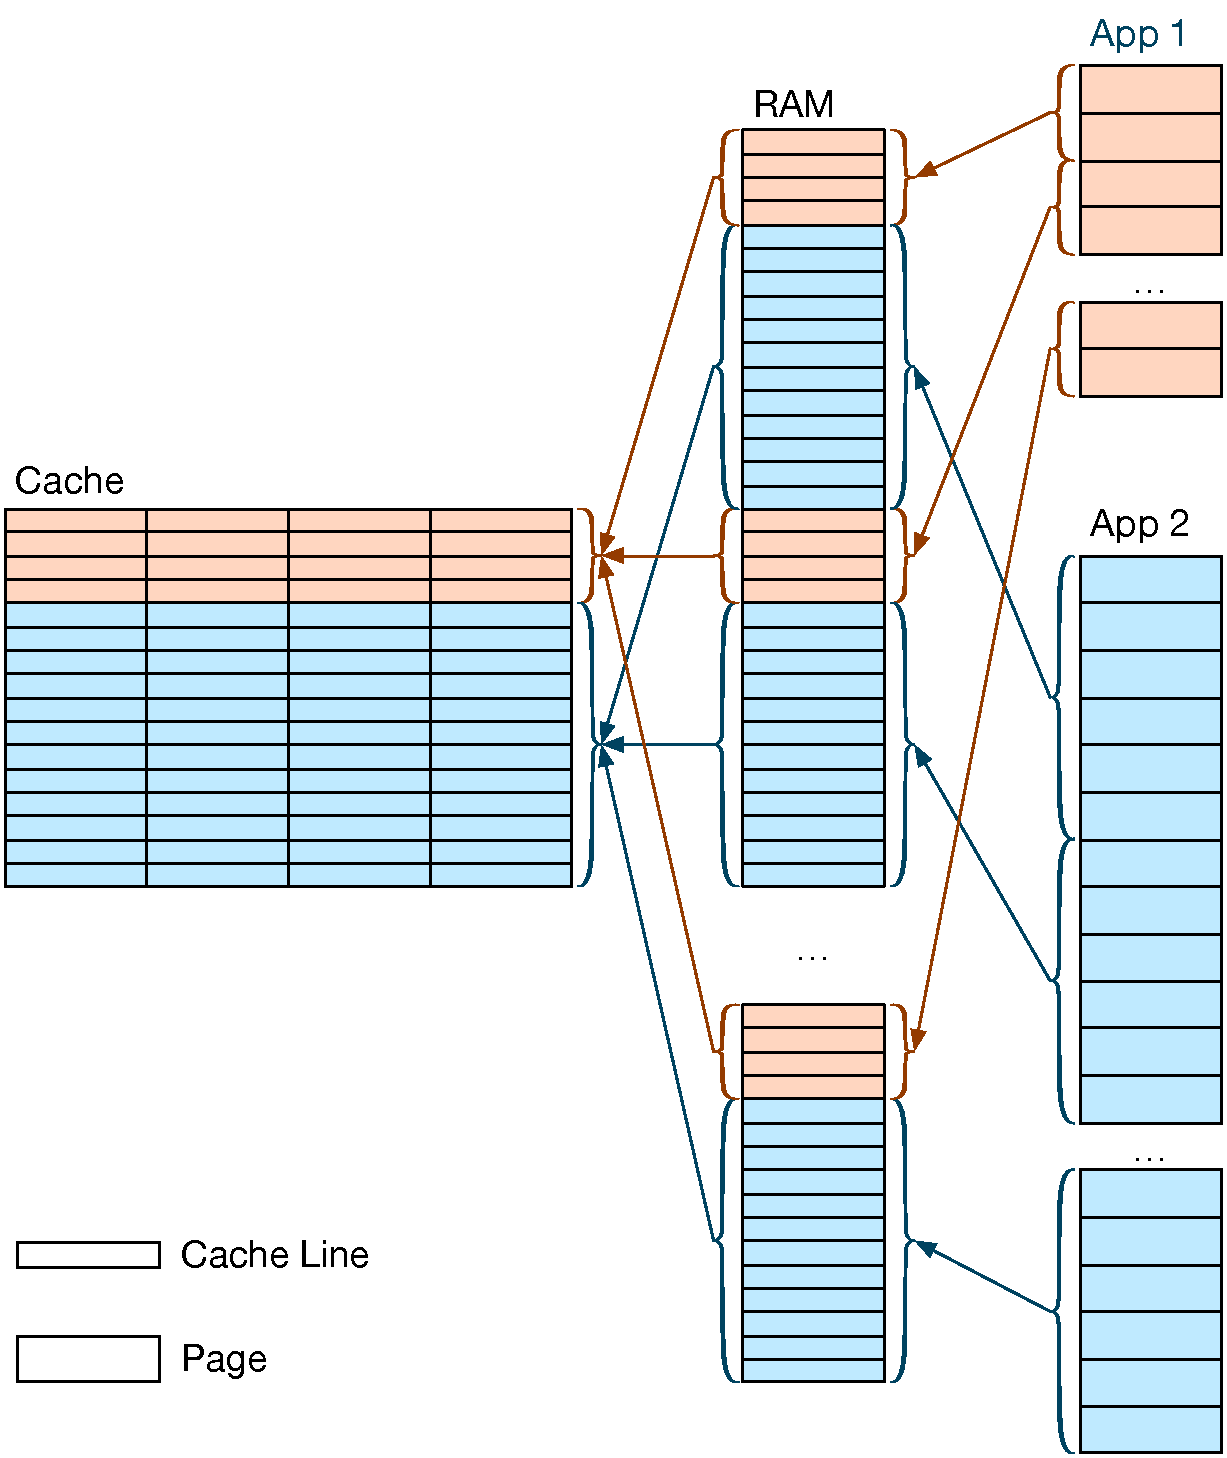
\includegraphics[width=85mm]{figures/cache_partitions.pdf}}
  \caption{
    Cache partitioning between two applications. Each application has some
    cache sets allocated to it, and only uses RAM regions that map to its cache
    sets. When partitioning the L1 cache, applications have to follow this
    constraint themselves. When the L2 cache is partitioned, the OS can map the
    pages in an application's virtual address space to the RAM regions that the
    application can use, so applications are oblivious to the cache
    partitioning.
  }
  \label{fig:cache_partitions}
\end{figure}


The scratchpad is used like a cache for the untrusted software's data. The
memory manager provides functions for reading and writing a memory location.
If the desired location is cached in the scratchpad, it is read or written
immediately. Otherwise, a cache line is evicted from the scratchpad, and
replaced with the line that contains the desired location. If evicted cache
line is dirty, it is written to the software's memory using an ORAM protocol.

To avoid leaking information via memory access timing, the memory manager
runs the ORAM protocol periodically, using the \texttt{RDTSC} instruction as
the clock source. On a read, the memory manager spins in a loop until it can
run the ORAM protocol. Writes are queued up, and the memory manager only spins
in a loop if the queue is full. The untrusted software must also periodically
call into our runtime, so it can run the ORAM protocol at the right time
even if no memory accesses are pending.

To remain future-proof, the memory manager uses the \texttt{CPUID} instruction
\cite{intel2013manual} to query the CPU's cache layout and aborts when faced
with an implementation that doesn't match our design assumptions.


\subsection{The Loader and Verifier}

We follow the approach of Google Native Client \cite{yee2009native}
\cite{sehr2010adapting}, namely we require that the untrusted software
satisfies some constraints that are easy to verify, and that guarantee that the
software will always interact with the outside world through our trusted
runtime. We provide a compiler that produces code meeting these constraints,
but the compiler is untrusted, and the software provider is free to replace our
compiler with any tool that produces code meeting our constraints. This results
in a small TCB, compared to rewriting the software's machine code on the fly,
and we expect that a technique similar to RockSalt \cite{morrisett2012rocksalt}
can be used to prove the correctness of our verifier.

The main constraint in our system is that untrusted software cannot contain
memory access instructions. All memory accesses must be performed by calling
into our memory manager. The software must also call into our memory manager
at the beginning of every basic block. Long basic blocks must call into our
runtime every 100 instructions\footnote{Exact number subject to tweaking}.

Our runtime hides the untrusted software's actual running time, to remove
information leak. Instead, the software's metadata specifies a deadline.
If the software does not meet the deadline, it is terminated. If it does, the
runtime spins until the deadline is reached. To implement this, we prohibit the
untrusted software from using \texttt{EEXIT} directly, and require that it
calls into our runtime instead. The periodic calls into the runtime metioned
above terminate the untrusted software if its deadline has passed.


\subsection{The Protected Environment}

SGX offers a protected environment for security-sensitive software, but the
environment leaks the memory access patterns (\S \ref{sec:sgx_leaks}). The
design described here needs stronger guarantees to prevent the attacks afforded
by our threat model.

The x86 address translation (\S \ref{sec:paging}) gives malicious system
software an opportunity to snoop on the enclave software, because of the
information reported by page faults. System software can also foil the cache
partitioning scheme used by our memory manager, because it controls some of the
bits in the physical memory addresses used to compute the cache set index. We
are exploring mechanisms for constraining the mapping of an enclave page to an
EPC page. The extra constraints would only be checked when an enclave page is
created (via \texttt{EADD}) or loaded into the EPC (via \texttt{ELDB}).

Asynchronous Enclave Exits (AEX) give malicious system software an opportunity
to preempt the enclave software and mount cache timing attacks. We are
investigating servicing faults inside the enclave, instead of performing an
AEX, and asking the local APIC to route interrupts to a different CPU if the
current CPU is executing enclave code. This approach would require the enclave
code to \texttt{EEXIT} in a timely manner, so the system software can schedule
other threads on the CPU. The deadline-enforcing mechanism in our runtime would
ensure that the untrusted software \texttt{EEXIT}s in time. The CPU would
prevent against malicious or buggy enclave code that loops forever by
implementing an inter-processor-interupt (IPI) that the system software could
issue from another CPU core to destroy the unresponsive enclave and flush the
core's caches.

AEX removal would make it impossible for the system software to take advantage
of hyper-threading to snoop on the enclave software by scheduling a malicious
thread on a logical processor in the same core as the logical processor
executing the enclave software. Our runtime would spin loop at start-up, until
the system software schedules enclave threads on all the logical processors
inside the core used to run enclave software. A simple approach would use one
thread to run enclave code, and spin loop on all the other threads. We are
also considering dedicating a logical processor to the ORAM protocol, and
another logical processor to running the untrusted software.


\setlength{\bibsep}{1pt}
\small
\bibliographystyle{plain}
%\bibliographystyle{abbrv}
\bibliography{references}

\end{document}
